\documentclass[11pt]{exam}
\usepackage[margin=1in]{geometry}
\pagestyle{plain}
\usepackage{amsmath,amsfonts,amssymb,amsthm,enumerate}
\usepackage{multicol}
\usepackage[]{graphicx}
\usepackage{hyperref}
\usepackage{tikz}
\usepackage{pgfplots}
\usepackage{subfigure}

\addtolength{\footskip}{2\baselineskip} % to lower the page numbers
\title{\vspace{-1.5in} Math 115 \\ Worksheet Section 1.6}
\date{}
\newcommand{\rJustifyAnswer}[1]{\ifprintanswers\hfill #1\phantom{\hspace{2in}} \fi}

% \theoremstyle{definition}
% \newtheorem{problem}{Problem}
\renewcommand{\questionlabel}{\textbf{Problem~\thequestion.}}
%\printanswers

\begin{document}
\maketitle
\vspace{-0.75in}
\begin{questions}
  \question
  \begin{parts}
   \part Every exponential \fillin[growth] function eventually
   dominates every \fillin[power function][1.4in].
   \part Consider the rational function $r(x) = \frac{p(x)}{q(x)}$. If the polynomials $p(x)$ and $q(x)$ have no common zeroes, then:
\begin{itemize}
\item Zeros of $p(x)$ give rise to \fillin[\(x\)-intercepts][3in].
\item Zeros of $q(x)$ give rise to \fillin[vertical asymptotes][3in].
\end{itemize}
\part When does $r(x)$ have an horizontal asymptote?
  \end{parts}
  \question Which function dominates as $x \to \infty$?
\begin{table}[h]\centering
\begin{tabular}{lll}
(a) $e^x$ or $10^{1000} \ln(x)$	& (b) $1000x^4$ or $0.2x^5$	& (c) $10e^{0.1x}$ or $5000x^2$\\ \\
(d) $100x^5$ or $1.05^x$	& (e) $x^4$ or $\ln(x)$	& (f) $e^x$ or $2.71^x$
\end{tabular}
\end{table}
\begin{solution}
  (a) \(e^x\), (b) \(0.2x^5\), (c) \(10e^{0.1x}\), (d) \(1.05^x\), (e)
  \(x^4\), (f) \(e^x\).
\end{solution}
\vspace{-0.1in}
\question Which of the following functions have the given properties?
\begin{table}[h]\centering
\begin{tabular}{lll}
(a) $y = \frac{x^2-2}{x^2+2}$	& (b) $y = \frac{x^2+2}{x^2-2}$	& (c) $y = (x-1)(1-x)(x+1)^2$\\ \\
(d) $y = x^3-x$	& (e) $y = x-\frac{1}{x}$	& (f) $y = (x^2-2)(x^2+2)$
\end{tabular}
\end{table}
\vspace{-0.1in}
\begin{enumerate}[(i)]
	\item A polynomial of degree 3. \rJustifyAnswer{(d)}
	\item A polynomial of degree 4. \rJustifyAnswer{(c), (f)}
	\item A rational function that is not a
          polynomial. \rJustifyAnswer{(a), (b), (e)}
	\item Exactly two distinct zeros. \rJustifyAnswer{(a), (c),
            (e), (f)}
	\item Exactly one vertical asymptote. \rJustifyAnswer{(e)}
	\item More than two distinct zeros. \rJustifyAnswer{(d)}
	\item Exactly two vertical asymptotes. \rJustifyAnswer{(b)}
	\item A horizontal asymptote. \rJustifyAnswer{(a), (b)}
\end{enumerate}
\begin{solution}
  The answers are written above. However, answers to (iv)--(viii) must be
  justified with work.
\end{solution}
\question (1.6 \#41--44) Assuming the window is large enough to show
end behavior, identify the graph as that of a rational function,
exponential function, or logarithmic function.\\
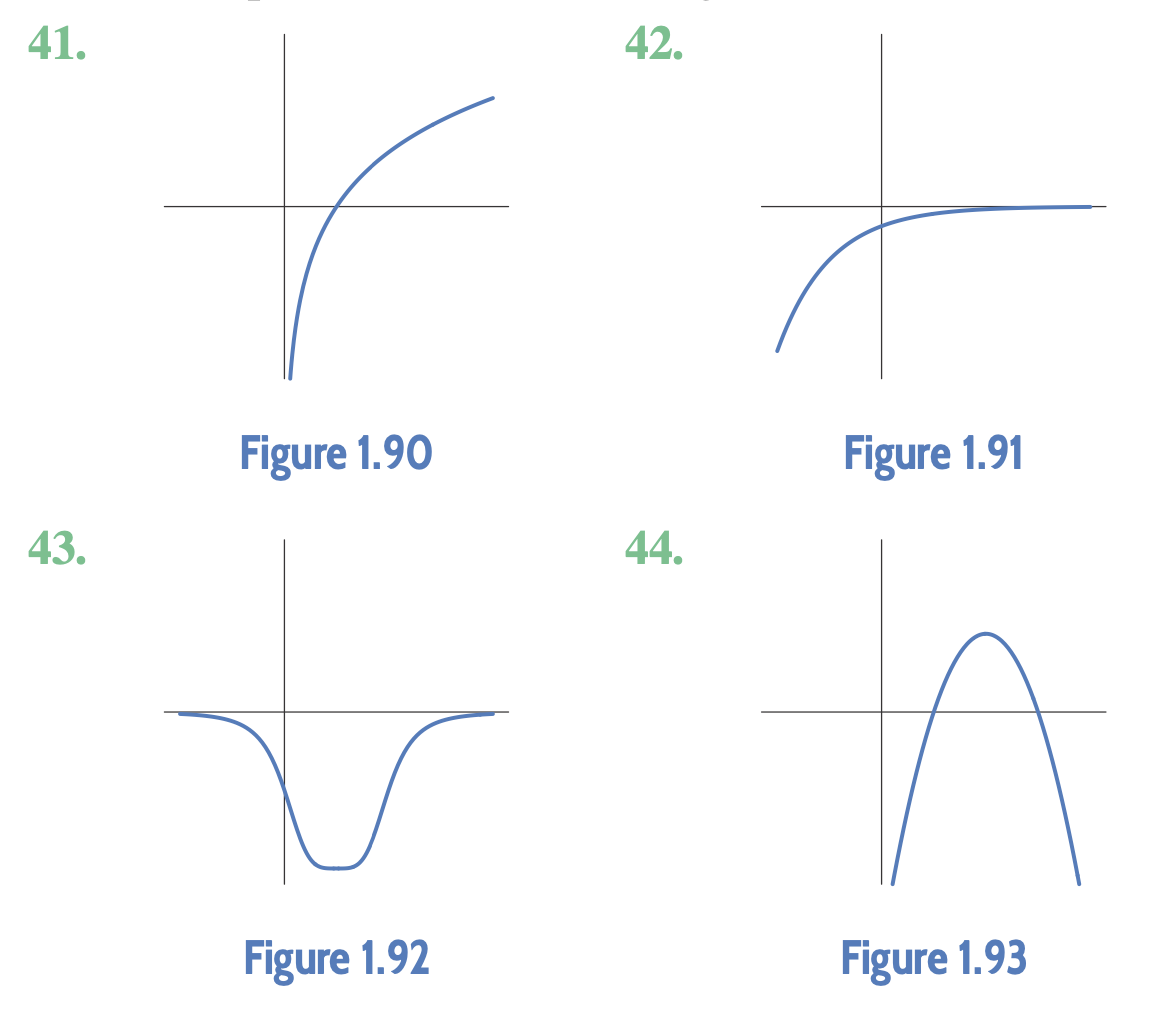
\includegraphics[scale=0.5]{Figures/probs41-44.png}
\begin{solution}
  Remember that rational functions may or may not have vertical
  asymptotes or a horizontal asymptote, but when they have vertical
  asymptotes, the function is defined on both sides of the asymptote. Also, when they
  have a horizontal asymptote, the function tends towards the
  horizontal asymptote both as \(x\to\infty\) and \(x\to-\infty\). Logarithmic
  functions have vertical asymptotes and no horizontal
  asymptotes and tend towards \(\pm\infty\) in one direction. Exponential functions have horizontal asymptotes but no
  vertical asymptotes and tend towards \(\pm\infty\) in one direction.
  \begin{enumerate}
  \item[41.]  Has a vertical asymptote and no horizontal
    asymptote. Furthermore, it has no values to the left of
    \(x=0\). Thus, it must be a logarithmic function.
  \item[42.]  Has a horizontal asymptote and no vertical
    asymptotes. Furthermore, the graph tends towards \(-\infty\) as
    \(x \to -\infty\). Thus, it must be an exponential function.
  \item[43.] This function has a horizontal asymptote and tends
    towards \(0\) both as \(x \to \infty\) and \(x \to
    -\infty\). Thus, it must be a rational function.
  \item[44.] This function has no asymptotes, but tends towards
    \(-\infty\) both as \(x \to \infty\) and \(x \to -\infty\). Thus,
    it must be a rational function.
  \end{enumerate}
\end{solution}
\question (Fall 2017 Exam 1)
Consider the rational function \(r\) defined by
$$r(x) = \frac{3(x-\sqrt{2})(\pi x + 7)^2(x+1)}{(x+1)(x-\sqrt{3})}.$$
For all of the following parts of this problem, leave your answers in exact form.
\begin{enumerate}[(a)]
\item What is the domain of $r(x)$?

\item Find the equations of all vertical asymptotes of $r(x)$. If there are none, write none.

\item Let $p(x) = x^2 + 1.2x -5$. Find the equations of all horizontal asymptotes of $\frac{r(x)}{p(x)}$. If there are none, write NONE. Show your work or reasoning to justify your answer.
\end{enumerate}
\begin{solution}
  See \href{https://dhsp.math.lsa.umich.edu/exams/115exam1/f17/s9.pdf}{https://dhsp.math.lsa.umich.edu/exams/115exam1/f17/s9.pdf}
\end{solution}
% Replace the following question?
\question (Winter 2017 Exam 1)
A group of students planted a pine tree and an oak tree alongside the Diag. Let $P(t)$ and $O(t)$ be the height (in feet) of the pine and the oak $t$ years after they were planted, where
$$P(t) = 170 - 165 A^{-0.02 t} \textrm{ and } O(t) = \frac{140}{2+100e^{-0.3t}}$$
where $A > 1$ is a constant. 
\begin{enumerate}[(a)]
\item How tall (in feet) were each of the trees when they were planted?
\item Ten years after the trees were planted, the height of the pine was 38 ft. Find the value of A. Find your answer algebraically and show all your work.
\item How many years after being planted does it take the oak to be 38 ft? Find your answer algebraically and show all your work.
\end{enumerate}
\begin{solution}
  See \href{https://dhsp.math.lsa.umich.edu/exams/115exam1/w17/s3.pdf}{https://dhsp.math.lsa.umich.edu/exams/115exam1/w17/s3.pdf} 
\end{solution}
\question Use a graphing calculator or Desmos to graph $y=x^4$ and $y = 3^x$. Determine approximate domains and ranges that give each of the graphs in the figure below.
	\begin{figure}[h]
	\centering
	\subfigure[]{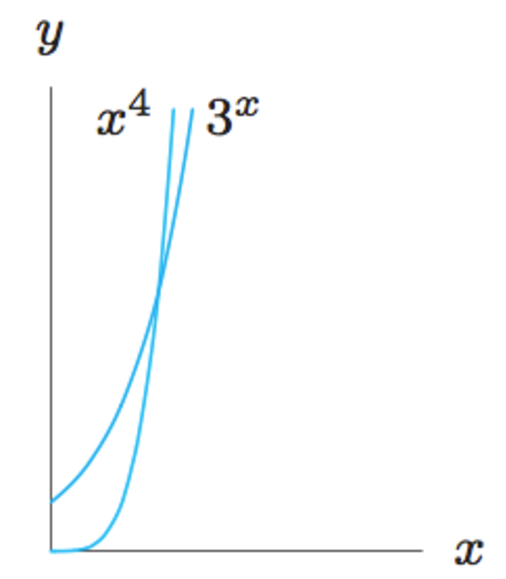
\includegraphics[scale=0.5]{Figures/fig3.pdf}}
	\subfigure[]{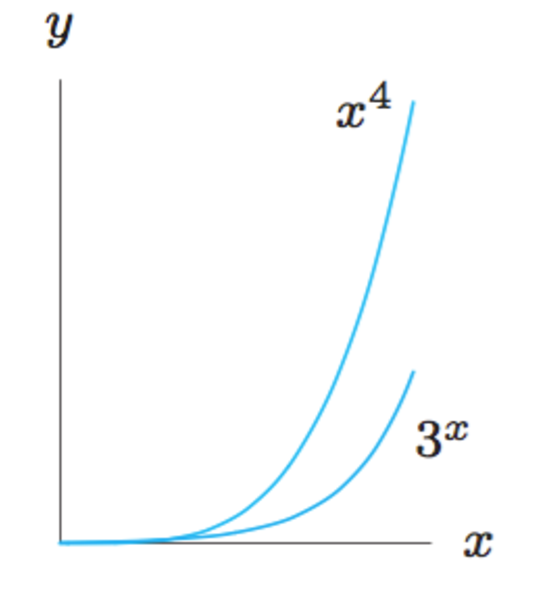
\includegraphics[scale=0.5]{Figures/fig4.pdf}}
	\subfigure[]{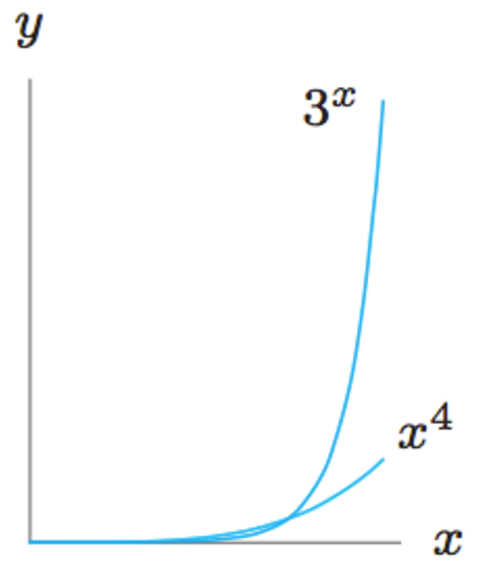
\includegraphics[scale=0.5]{Figures/fig5.pdf}}
	\end{figure}
\begin{solution}
  Values are very approximate. The important thing is to see that
  the relationship between the two functions looks different on different scales here.\\
  (a) Domain: \([0,2]\), Range: \([0,10]\) (b) Domain: \([0,4]\),
  Range: \([0,250]\) (c) Domain: \([0,10]\), Range: \([0,100000]\).
\end{solution}
\end{questions}
\end{document}
%%% Local Variables:
%%% mode: latex
%%% TeX-master: t
%%% End:
